\begin{figure}[htbp]
  \centering
  \begin{subfigure}[t]{0.48\linewidth}
    \centering
    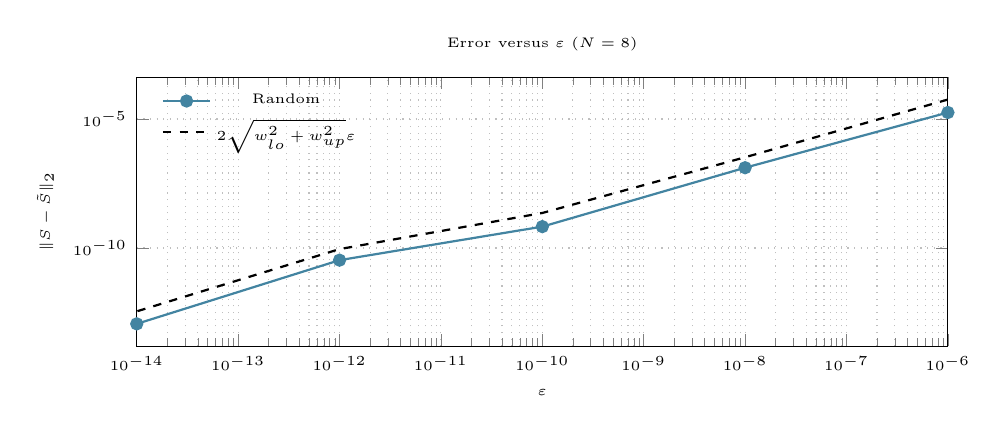
\begin{tikzpicture}
    \begin{axis}[
        width=0.98\linewidth,
        height=5.0cm,
        grid=both,
        grid style={dotted},
        minor tick num=0,
        enlarge x limits=false,
        xlabel near ticks,
        ylabel near ticks,
        xlabel style={font=\tiny},
        ylabel style={font=\tiny},
        tick label style={font=\tiny},
        legend style={
            font=\tiny,
            draw=none,
            fill=none,
            at={(0.02,0.98)},
            anchor=north west,
        },
        xmode=log,
        ymode=log,
        log basis x=10,
        xlabel={$\varepsilon$},
        ylabel={$\|S-\tilde S\|_2$},
        title={\tiny{Error versus $\varepsilon$ ($N=8$)}},
    ]
    \addplot[cyan!60!black, thick, mark=*] coordinates{
    (1.000000e-06, 1.787423e-05) (1.000000e-08, 1.295686e-07) (1.000000e-10, 6.756863e-10) (1.000000e-12, 3.393947e-11) (1.000000e-14, 1.155286e-13)
    }; \addlegendentry{Random}
    \addplot[black, dashed, thick, mark=none] coordinates{
    (1.000000e-06, 5.678374e-05) (1.000000e-08, 3.297979e-07) (1.000000e-10, 2.286000e-09) (1.000000e-12, 9.105410e-11) (1.000000e-14, 3.521653e-13)
    }; \addlegendentry{$2\sqrt{w_{lo}^2+w_{up}^2}\varepsilon$}
    \end{axis}
    \end{tikzpicture}
\caption{For $N=8$ we report how the block encoding error increases with $\varepsilon$ ranging from 1.0e-14 to 1.0e-06.
        \label{fig:first}}
  \end{subfigure}
  \hfill
  \begin{subfigure}[t]{0.48\linewidth}
    \centering
    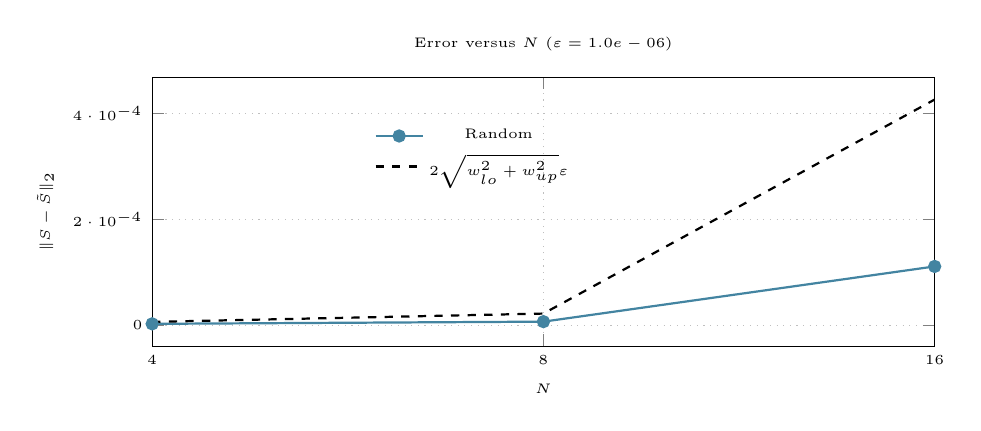
\begin{tikzpicture}
    \begin{axis}[
        width=0.95\linewidth,
        height=5.0cm,
        grid=both,
        grid style={dotted},
        minor tick num=0,
        enlarge x limits=false,
        xlabel near ticks,
        ylabel near ticks,
        xlabel style={font=\tiny},
        ylabel style={font=\tiny},
        tick label style={font=\tiny},
        legend style={
            font=\tiny,
            draw=none,
            fill=none,
            at={(0.55,0.85)},
            anchor=north east,
        },
        xmode=log,
        log basis x=2,
        xmin=4, xmax=16,
        xtick={4,8,16},
        xticklabels={4,8,16},
        xlabel={$N$},
        ylabel={$\|S-\tilde S\|_2$},
        title={\tiny{Error versus $N$ ($\varepsilon=1.0e-06$)}},
        scaled y ticks=false,
    ]
    \addplot[cyan!60!black, thick, mark=*] coordinates{
    (4.000000e+00, 2.300516e-06) (8.000000e+00, 6.442899e-06) (1.600000e+01, 1.108780e-04)
    }; \addlegendentry{Random}
    \addplot[black, dashed, thick, mark=none] coordinates{
    (4.000000e+00, 5.987432e-06) (8.000000e+00, 2.173163e-05) (1.600000e+01, 4.265265e-04)
    }; \addlegendentry{$2\sqrt{w_{lo}^2+w_{up}^2}\varepsilon$}
    \end{axis}
    \end{tikzpicture}
            \caption{For different values of $N$ and for $\varepsilon = 1.0e-06$, we report the actual errors of the encoding for the Random generator case, together with the theorem bound $2\sqrt{w_{lo}^2+w_{up}^2}\varepsilon$.}
        \label{fig:second}
  \end{subfigure}
  \caption{Unsymmetric semiseparable reconstruction error scaling: sensitivity to $\varepsilon$ (left) and $N$ (right).}
  \label{fig:err_combined_unsymm}
\end{figure}
